Il modulo inerente agli aspetti di computer vision � stato realizzato mediante l'uso di una telecamera RGB-D, in particolare tramite una {\itshape Microsoft Kinect}, il cui stream video � stato processato con l'ausilio dell'API {\itshape OpenCV}.\newline
Il modulo di visione in questione prevede la realizzazione della seguente pipeline:
\begin{enumerate}
	\item acquisizione dello stream video RGB e di profondit� e conversione dello spazio di colore da RGB a HSV;
	\item ricerca del blob di massima dimensione del colore target associato alla sessione corrente;
	\item estrazione del valore di profondit� associato al centroide del blob;
	\item calcolo del vettore in direzione del target.
\end{enumerate}
\subsection{Acquisizione dello stream video}
L'acquisizione dello stream video tramite camera RGB-D � stata realizzata mediante l'uso del framework open-source {\itshape OpenNI}, ideato per accedere alle informazioni registrate dalla camera con un livello di astrazione alto. In particolare, l'acquisizione dello stream video RGB � stata realizzata attraverso la sottoscrizione al topic \texttt {/camera/rgb/image\_rect\_color} mentre l'acquisizione dello stream video di profondit� � stata realizzata attraverso la sottoscrizione al topic \\
\texttt {/camera/depth\_registered/image}.

Siccome entrambi i topic forniscono informazioni mediante messaggi di tipo \texttt{sensor\_msgs/Image}, per permettere l'analisi tramite {\itshape OpenCV} � necessario convertire entrambi gli stream video nel formato \texttt {cv::Mat}. La suddetta conversione � stata realizzata mediante l'uso della libreria {\itshape CvBridge} con la seguente funzione di conversione
\begin{center}
	\texttt{imgmsg\_to\_cv2(frame\_video, encoding)}
\end{center}
dove per encoding sono stati utilizzati \texttt{bgr8} ed \texttt{32FC1} rispettivamente per la conversione dell'immagine RGB e di profondit�.

\begin{figure}[htbp]
	\begin{center}
		\subfigure[Frame RGB\label{fig:RGBimg}]{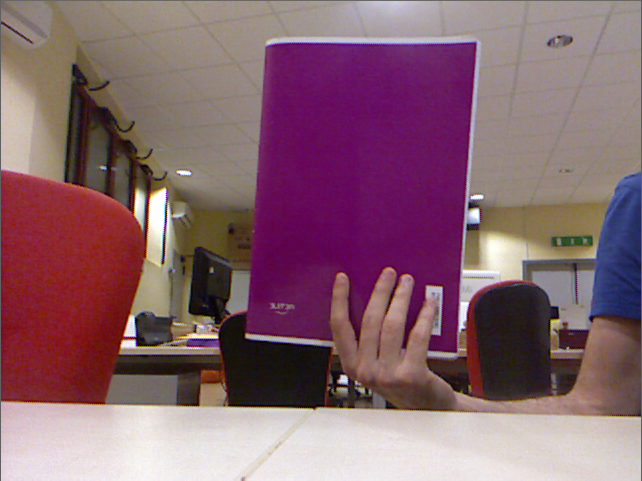
\includegraphics[width=55mm]{images/1-RGB.png}}
		\subfigure[Frame Depth\label{fig:depthImg}]{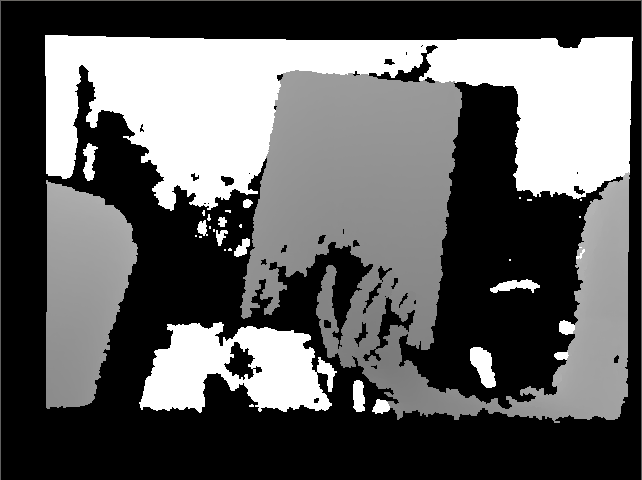
\includegraphics[width=55mm]{images/2-Depth.png}}
	\end{center}
\end{figure}

Per agevolare l'analisi dei frame � stato effettuato un preprocessing dei frame RGB in cui � prevista l'applicazione di un filtro gaussiano (per rimuovere l'eventuale presenza di rumore video) realizzato mediante l'uso di un kernel di dimensioni \texttt{3x3}. L'applicazione del suddetto filtro � stata ottenuta mediante l'uso della funzione \texttt{cv2.GaussianBlur()}.

Essendo questa fase fortemente soggetta ad una discriminazione dei colori presenti nei frame, � stata effettuata una conversione dello spazio di colori da \texttt{RGB} a \texttt{HSV} mediante la funzione \texttt{cv2.cvtColor()}. Cos� facendo viene gestita in maniera pi� "naturale" la distinzione dei colori, in quanto nello spazio HSV la variazione dei colori � soggetta soltanto alla componente {\itshape Hue} a differenza dello spazio RGB, in cui un colore viene visto come una combinazione di rosso, giallo e blu.

\subsection{Estrazione del blob e calcolo del centroide}
La {\itshape palette} dei colori a disposizione nel gioco � stata realizzata mediante l'uso di intervalli di colore espressi in formato HSV. Ad ogni colore quindi � associato un intervallo e durante la fase di estrazione del colore, ogni valore contenuto nell'intervallo associato al colore target � considerato valido.

Per realizzare tale selezione � stata utilizzata la funzione
\begin{center}
	\texttt{cv2.inRange(frame\_video, lower\_bound, upper\_bound)}
\end{center} 
dove per \texttt{lower\_bound} ed \texttt{upper\_bound} sono stati inseriti gli estremi dell'intervallo associati al colore target. Dalla funzione viene ritornata una maschera il cui scopo � di isolare dal frame corrente soltanto le informazioni utili alla ricerca del blob.

\begin{figure}[htbp]
	\begin{center}
		\subfigure[Maschera\label{fig:RGBimg}]{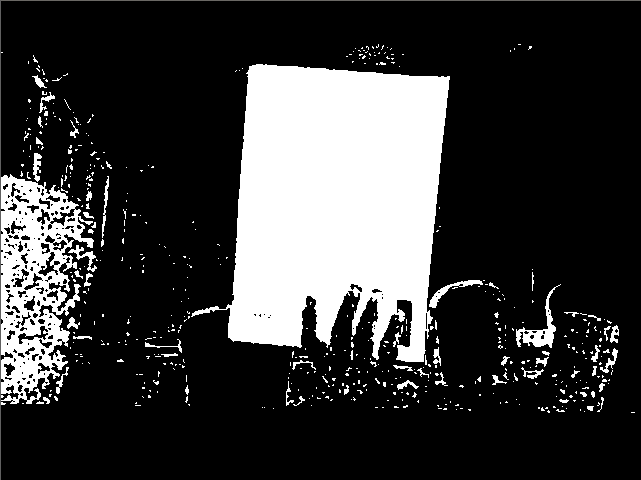
\includegraphics[width=55mm]{images/3-Mask.png}}
	\end{center}
\end{figure}

Tuttavia la maschera evidenzia anche piccole porzioni di immagine che possono deviare la corretta ricerca del blob e che quindi costituiscono un rumore. Per eliminare gran parte di tale rumore � stata effettuata un'operazione di {\itshape erosione} tramite l'uso della funzione \texttt{cv2.erode()} seguita da un'operazione di {\itshape dilatazione} tramite l'uso della funzione \texttt{cv2.dilate()} utile a ristabilire le proporzioni delle componenti utili evidenziate dalla maschera.

\begin{figure}[htbp]
	\begin{center}
		\subfigure[Erosione\label{fig:erosion}]{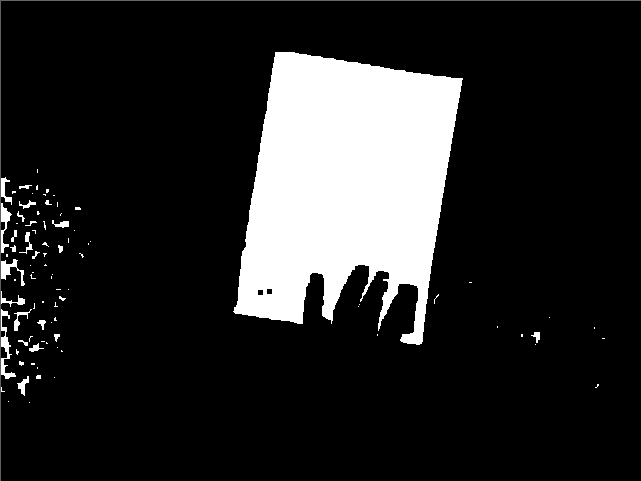
\includegraphics[width=55mm]{images/4-erode.png}}
		\subfigure[Dilatazione\label{fig:dilatation}]{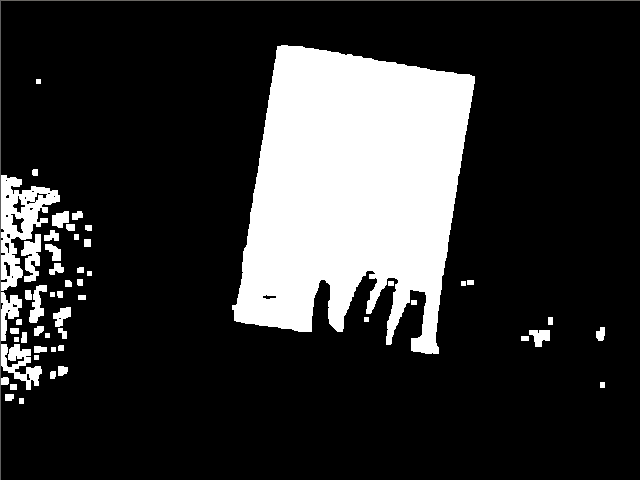
\includegraphics[width=55mm]{images/5-dilate.png}}
	\end{center}
\end{figure}

Per tener traccia dei blob presenti nella scena, � stata utilizzata la funzione
\begin{center}
	\texttt{cv2.findContours(mask, cv2.RETR\_EXTERNAL, cv2.CHAIN\_APPROX\_SIMPLE)}
\end{center}
dove \texttt{cv2.RETR\_EXTERNAL} indica che vengono estratti soltanto i contorni esterni (trascurando quindi i contorni innestati in altri), mentre \texttt{cv2.CHAIN\_APPROX\_SIMPLE} indica che viene realizzata un'ottimizzazione dello spazio necessario a memorizzare i contorni.

Successivamente viene selezionato il blob avente area maggiore e, tramite la funzione \texttt{cv2.minEnclosingCircle()}, viene estratto il raggio del cerchio di area minima che lo include. Il blob in questione viene considerato valido soltanto se avente raggio superiore ad una soglia fissata apriori.

Arrivati a questo punto, viene estratto il centroide mediante i {\itshape momenti dell'immagine} associati al contorno del blob tramite la funzione \texttt{cv2.moments(contour)}. In particolare, le coordinate che identificano il centroide sono cos� espresse:
\begin{center}
	$C_x=\frac{M_{10}}{M_{00}}$, $C_y=\frac{M_{01}}{M_{00}}$
\end{center}

\begin{figure}[htbp]
	\begin{center}
		\subfigure[Blob selezionato\label{fig:RGBimg}]{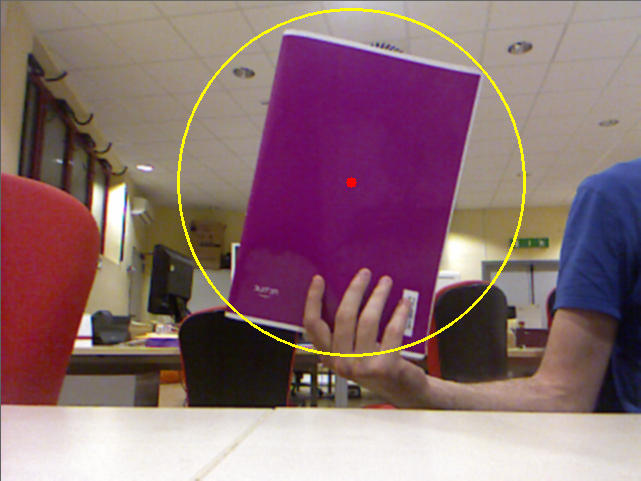
\includegraphics[width=55mm]{images/6-final.png}}
	\end{center}
\end{figure}

\subsection{Estrazione della profondit�}
Giunti a questa fase, si ha a disposizione il centroide rappresentante il target da seguire. Possiamo quindi estrarre la distanza del blob dalla camera utilizzando la componente di profondit� processata dalla camera RGB-D.

L'immagine di profondit� a disposizione � nel formato \texttt{cv::Mat}, quindi per accedere alla distanza al centroide del blob � sufficiente estrarre dall'immagine la componente $(C_x,C_y)$. Cos� facendo si otterr� un valore in {\itshape floating point} a 32 bit rappresentante la distanza in metri del punto osservato nel pixel dalla camera.

\subsection{Calcolo della direzione da seguire}
Per ottenere il vettore in direzione del target � stato utilizzato il raggio uscente dalla camera ed entrante nel pixel che costituisce il centroide del target.\newline
Essendo l'immagine ottenuta per proiezione prospettica della scena visualizzata dalla camera su di un piano di proiezione, il raggio ottenuto potr� essere considerato valido per la generazione del vettore direzionale che vogliamo realizzare.

� stato utilizzato quindi il modello della {\itshape Pin-hole camera} per elaborare le informazioni associate alla Kinect ed estrarre il raggio in questione. Tali informazioni vengono estratte dal topic \texttt{/camera/depth\_registered/camera\_info} sottoforma di messaggio \texttt{sensor\_msgs/CameraInfo}.
Il modello della camera viene realizzato mediante l'uso dell'oggetto \texttt{PinholeCameraModel} contenuto nella libreria \texttt{image\_geometry} nativa di ROS.
Successivamente, mediante la funzione
\begin{center}
	\texttt{projectPixelTo3dRay(centroid)}
\end{center}
viene estratto il raggio uscente dalla camera in direzione della coppia di coordinate $C_x,C_y$ sottoforma di versore. Infine, dalla moltiplicazione delle componenti $x,z$ del raggio appena ottenuto con la distanza estratta allo step precedente, viene generato il vettore direzionale utile al robot per raggiungere il target.
